\chapter[Integrated genomic and transcriptomic analysis of small cell lung cancer]{Integrated genomic and transcriptomic analysis of small cell lung cancer\footnote{This chapter currently accepted for publication as: Chen HZ\cofirst, Bonneville R\cofirst, Paruchuri A\cofirst, \textit{et al}. Genomic and transcriptomic characterization of relapsed small cell lung cancer through rapid research autopsy. \textit{JTO Clinical and Case Reports}.}}
\label{ch:sclc}

\section{Introduction}
Small cell lung cancer (SCLC) is a lethal neuroendocrine malignancy accounting for 13--15\% of new lung cancer cases annually worldwide \cite{sabari2017,siegel2019}. Most SCLC patients present with initially chemotherapy-sensitive disease, but almost all will experience progression or relapse leading to death. In 2019, combination chemotherapy and immunotherapy was FDA-approved as first-line treatment for metastatic SCLC \cite{horn2018,pazares2019}, with modest two-month improvement in survival compared to chemotherapy alone. For decades, topotecan was the only FDA-approved second-line chemotherapy with objective response rate (ORR) of 10--20\% \cite{pawel1999}, until lurbinectedin was granted accelerated approval in 2020 based on a phase II trial showing 35\% ORR \cite{trigo2020}. Despite these recent approvals, there is an urgent need to develop more effective therapies for advanced SCLC\@.

Key studies in the last decade have profiled the mutational landscape of primary SCLC, driven by \textit{TP53} and \textit{RB1} inactivation \cite{george2015,rudin2012,peifer2012}. Furthermore, distinct SCLC subgroups have been identified based on the expression of key transcription factors including ASCL1 and NEUROD1 \cite{rudin2019,baine2020}. How each SCLC subtype confers different clinical phenotypes and differential response to anti-cancer therapies is under active investigation \cite{gay2021}, with the goal of delivering precision therapy to SCLC patients by matching each SCLC subtype to specific treatments. 

Molecular characterization of relapsed SCLC has been hampered by tissue scarcity due to rapid clinical deterioration of relapsed patients. Therefore, unlike for primary SCLC, less is known about the genomic and transcriptomic landscapes of relapsed SCLC and mechanisms that mediate therapeutic resistance, although recent non-autopsy studies on relapsed SCLC have begun to address this knowledge gap. For example, Gardner \textit{et al} used patient-derived xenografts of paired chemosensitive and chemoresistant SCLC tumors to elegantly demonstrate that acquired chemoresistance occurred through epigenetic silencing of a DNA damage repair factor, \textit{SLFN11} \cite{gardner2017}. Wagner \textit{et al} performed genomic profiling on a cohort of relapsed SCLC patients and identified recurrent Wnt pathway alterations as a mechanism of acquired chemoresistance \cite{wagner2018}. Weiss \textit{et al} performed genome-wide exome and RNA-seq on twelve SCLC patients who relapsed after platinum-based chemotherapy \cite{weiss2017}. Aside from driver mutations in \textit{RB1} and \textit{TP53}, the authors identified few recurrent targetable genomic alterations in this cohort of patients. Finally, an important study by Stewart \textit{et al} performed single cell sequencing of circulating tumor cells (CTCs) and CTC-derived xenografts from platinum-sensitive and refractory SCLC patients and demonstrated an association between increased intratumoral heterogeneity and chemoresistance \cite{stewart2020}. The latter study is one of the first non-autopsy studies to directly evaluate intratumor heterogeneity in advanced SCLC\@. Overall, however, further study of relapsed SCLC is needed to identify additional targetable mechanisms underlying therapeutic resistance, including resistance to immunotherapy which is now approved for front-line treatment in the metastatic setting. 

The utilization of tumor specimens from rapid research autopsy has accelerated the study of tumor heterogeneity and acquired resistance in advanced cancer (Section~\ref{ssec:intro:heterogeneity_methods}) \cite{krook2019_review}. To our knowledge, this is the first study to perform whole exome and transcriptome profiling of advanced SCLC through research autopsy. From exome sequencing, we inferred intertumor and intratumor clonal heterogeneity arising from branched and linear evolution, while transcriptome analyses supported the subtype-specific suppression of adaptive anti-tumor immunity in primary and advanced SCLC\@. Our results provide new insights into the subclonal architecture of advanced SCLC and identify new potentially targetable pathways involved in anti-tumor immune responses.

\section{Materials and Methods}
\subsection{Rapid research autopsy}
Informed consents were obtained from five patients with advanced SCLC to participate in an IRB-approved clinical study for tumor profiling by next-generation sequencing (NGS) and body donation (NCT02090530) \cite{krook2019_review,krook2019_mcs}. Deceased patients were transported to The Ohio State University Regional Autopsy Center, where research autopsy for tumor procurement was performed no more than 16 hours after patients' passing. CT imaging when available was used to guide procurement from organs with cancer. After autopsy completion, the deceased were transported to a designated funeral home within 24 hours.

\subsection{Tumor DNA/RNA sequencing}
Samples with tumor cell content \textgreater{}60\% and without significant necrosis were selected for NGS analyses. Genomic DNA and total RNA were extracted using Qiagen kits per manufacturer's protocol. Libraries were prepared following established protocols (TruSeq Stranded Total RNA with Ribo-Zero Gold\textsuperscript\textregistered{} from Illumina) \cite{krook2019_mcs,reeser2017}, enriched with the xGEN Exome Research Panel v1.0 (IDT), and sequenced on an Illumina HiSeq 4000.

In addition, we utilized RNA-seq data of primary and relapsed SCLC and normal lung tissue obtained from previous publications \cite{rudin2012,wagner2018,weiss2017,fagerberg2014}. Of these data sets, one had paired primary SCLC and normal lung samples \cite{rudin2012}, while the rest contained either exclusively tumor \cite{wagner2018,weiss2017} or normal samples \cite{fagerberg2014}. Non-SCLC RNAseq data \cite{tcgaluad,tcgalusc} were downloaded from The Cancer Genome Atlas via the Genomic Data Commons (GDC) data portal (\url{https://portal.gdc.cancer.gov/}). We randomly chose a subset of 60 and 49 tumor-normal paired samples of lung adenocarcinoma and squamous cell carcinoma, respectively, for ssGSEA and ImSig analyses.

\subsection[ctDNA sequencing]{Circulating tumor DNA (ctDNA) sequencing}
ctDNA was isolated using QIAamp Circulating Nucleic Acid Kit per manufacturer's protocol. An input of 300~ng was used to generate libraries for paired-end sequencing on a NextSeq instrument achieving median coverage of \textapprox{}500\texttimes{} \cite{griffith2015}.

\subsection[SNVs and CNVs, clonal inference, and mutational signatures]{Somatic mutation and copy number variant calling, clonal inference, and mutational signatures}
These bioinformatics analyses were performed as previously described (Section~\ref{sec:240:methods}). Briefly, sequencing reads were aligned to hg19 using bwa \cite{bwa}, deduplication performed with Picard \cite{Picard2019toolkit}, and base quality score recombination and realignment around indels with GATK \cite{mckenna10}. Variants were called with VarScan2 \cite{varscan2} and allele-specific CNVs with FALCON \cite{falcon}. Clonal inference was performed using Canopy \cite{canopy}, and mutational signatures were inferred with deconstructSigs \cite{rosenthal16}. Bradley-Terry modeling was used to estimate relative ordering of mutations in the phylogeny branches of SCLC autopsy patients as previously described (Section~\ref{ssec:240:mutational_ordering}).

\subsection{Clonal fraction estimation in ctDNA}
\label{ssec:sclc:ctdna_clones}
\subsubsection{Definitions}
\newcommand*{\CM}{\mathbf{\tilde{C}^\text{M}}}
\newcommand*{\Cm}{\mathbf{\tilde{C}^\text{m}}}
To be solved is the probability vector $\hat{\theta}$ such that:
\begin{equation}
    \hat{\theta} = \argmax_{\vec\theta} \mathcal{L}\left(\vec{\theta} | \vec{r}, \vec{x},\vec{W}^\text{M}, \vec{W}^\text{m}, \vec{\varepsilon}^\text{M}, \vec{\varepsilon}^\text{m}, \CM, \Cm, f(m,\vec{\theta})\right)
\end{equation}
where $\hat{\theta} \in \mathbb{R}^K$ is the fraction of normal ($k=1$) and each clone $k-1$ for $k=2..K$. As a probability vector, all elements of $\vec\theta \ge 0$, and $||\vec\theta||_1 = 1$.

From Canopy output, we obtain:

\startsinglespace
\begin{description}[noitemsep]
    \renewcommand{\makelabel}[1]{#1:}
    \item[$M$] set of mutations included in the phylogenetic tree obtained by Canopy from autopsy samples (\emph{not} including \textit{post hoc} assignment)
    \item[$N=|M|$] number of these mutations
    \item[$T$] number of curated copy number variation (CNV)-affected regions from autopsy samples
    \item[$\CM \in \mathbb{Z}^{T \times K}$] major copy number of each CNV-affected region in each clone (and normal)
    \item[$\Cm \in \mathbb{Z}^{T \times K}$] minor copy number of each CNV-affected region in each clone (and normal)
    \item[$f(m,\theta) \in {[0..1]}$] given the Canopy-derived phylogenetic tree, the expected VAF of mutation $m \in M$ given clonal fractions $\theta$
\end{description}
\startdoublespace

From the ctDNA sample, we obtain:
\startsinglespace
\begin{description}[noitemsep]
    \renewcommand{\makelabel}[1]{#1:}
    \item[$\vec{r} \in \mathbb{Z}^N$] alternative-supporting reads for each mutation
    \item[$\vec{x} \in \mathbb{Z}^N$] depth of coverage for each mutation
    \item[$\vec{W}^\text{M} \in \mathbb{R}^T$] major copy number (CN) of curated CNV-affected regions in the ctDNA sample
    \item[$\vec{W}^\text{m} \in \mathbb{R}^T$] minor CN of curated CNV-affected regions
    \item[$\vec{\varepsilon}^\text{M} \in \mathbb{R}^T$] standard deviations of major CNs
    \item[$\vec{\varepsilon}^\text{m} \in \mathbb{R}^T$] standard deviations of minor CNs
\end{description}
\startdoublespace

\subsubsection{Expected VAF given tree}
Calculation of $f(m,\theta)$ for given $m \in M$ and $\theta$ requires several steps. From Canopy, we also have $\mathbf{H} \in \{0, 1\}^{N \times T}$ such that:
\begin{equation*}
    H_{mt} = \begin{cases}
        1 & \text{if mutation } m \text { is on major allele of CNA } t \\
        0 & \text{otherwise}\\
        \end{cases}
\end{equation*}

We compute $\vec{a} \in \mathbb{R}^{T}$, the total CN of all CNV-affected regions in the ctDNA sample given $\theta$:
\begin{equation*}
    \vec{a} = (\CM + \Cm)\theta
\end{equation*}

Next, we calculate the CN of $m$ in each subclone, $\vec{b} \in \mathbb{Z}^K$:
\begin{equation*}
    b_k = \begin{cases}
        0 & \text{if subclone } k \in K \text{ does not contain } m \\
        1 & \text{if } m \text{ is not within or is after a CNV in subclone } k \\
        \tilde{C}^\text{M}_{tk} & \text{if } m \text{ in CNV } t \text{ and } H_{mt} = 1 \\
        \tilde{C}^\text{m}_{tk} & \text{if } m \text{ in CNV } t \text{ and } H_{mt} = 0
    \end{cases}
\end{equation*}
and the copy number of $m$ in the ctDNA sample:
\begin{equation*}
    s = \theta^\mathsf{T} \vec{b}
\end{equation*}

We next compute the total CN of $m$'s position in the ctDNA sample:
\begin{equation*}
    c = \begin{cases}
        a_t & \text{if } m \text{ in CNV } t \\
        2 & \text{if } m \text{ not in a CNV}
    \end{cases}
\end{equation*}
Note that the patient's sex does not need to be considered, as only autosomal mutations were supplied to Canopy for tree building.

Now, computation of $f(m, \theta)$ is straightforward:
\begin{equation}
    f(m, \theta) = \frac{s}{c}
\end{equation}

\subsubsection{Likelihood function}
Analogous to Canopy, we model major and minor CN as normally distributed, and alternate-supporting reads as binomially distributed. We compute $\vec{g}^\text{M} \in \mathbb{Z}^T$, the expected major CN for each region $t \in T$ given $\vec\theta$, along with $\vec{g}^\text{m} \in \mathbb{Z}^T$ the expected minor CNs, as follows:
\begin{align*}
    \vec{g}^\text{M} &= \CM \vec\theta \\
    \vec{g}^\text{m} &= \Cm \vec\theta
\end{align*}

We construct the likelihood function for $\vec{\theta}$ as follows:
\begin{multline}
    \mathcal{L}\left(\vec{\theta} | \vec{r}, \vec{x},\vec{W}^\text{M}, \vec{W}^\text{m}, \vec{\varepsilon}^\text{M}, \vec{\varepsilon}^\text{m}, \CM, \Cm, f(m,\vec{\theta})\right) = \\
    \prod_{m \in M}\left(\pBinom\left(r_m, x_m, f(m, \vec{\theta})\right)\right) \cdot \prod_{t \in T}\left(\pNorm(W^\text{M}_t, g^\text{M}_t, \varepsilon^\text{M}_t) \pNorm(W^\text{m}_t, g^\text{m}_t, \varepsilon^\text{m}_t)\right)
\end{multline}
where $\pBinom(x, n, p)$ is the probability mass function at $x$ of a binomial distribution with $n$ trials and $p$ probability of success, and $\pNorm(x, \mu, \sigma)$ is the probability distribution function at $x$ of a normal distribution with mean $\mu$ and standard deviation $\sigma$. With log transformation, this becomes:
\begin{align}
    &\ln(\mathcal{L}(\vec\theta | \ldots) \nonumber \\
    &= \sum_{m \in M} \left( \sum_{j=r_m+1}^{x_m} \ln(j) - \sum_{j=1}^{x_m-r_m}\ln(j) + r_m\ln\left(f(m,\vec{\theta})\right) + (x_m-r_m)\ln\left(1-f(m,\vec{\theta})\right)\right) \nonumber \\
    &\phantom{=} - \frac{1}{2}\sum_{t \in T} \left( \left(\frac{W^\text{M}_t - g^\text{M}_t}{\varepsilon^\text{M}_t}\right)^2 + \left(\frac{W^\text{m}_t - g^\text{m}_t}{\varepsilon^\text{m}_t}\right)^2 + 2\ln(2\pi \varepsilon^\text{M}_t \varepsilon^\text{m}_t)\right)
\end{align}

\subsubsection{Optimization of likelihood}
We apply simulated annealing \cite{metropolis53,kirkpatrick83} to approximate $\hat\theta$. We begin by randomly initializing $\vec\theta_0$, with our current best $\hat\theta = \vec\theta_0$. Given hyperparameters $t_\text{max} = 25000$ (number of iterations), $\eta_0 = 0.2$ (initial learning rate), $\eta_\text{max} = 0.01$ (final learning rate), and $\rho = 25$ (suboptimal jump suppression), we implement this approach as follows: \\
\begin{minipage}{0.8\textwidth}
    \begin{algorithm}[H]
        \caption{Training of $\hat\theta$}
        \begin{algorithmic}[1]
            \For {$t \in 1..t_{max}$}
                \State $\vec\theta_t \gets \vec\theta_{t-1}$
                \State $l_1, l_2 \gets$ two random positions within $\vec\theta_t$
    			\State $x \gets \vec\theta_{t\,l_1}$, $y \gets \vec\theta_{t\,l_2}$ \Comment{Redistribute probabilities of $\vec\theta_{t\,l_1}$ and $\vec\theta_{t\,l_2}$}
    			\State $s \gets x+y$, $x \gets \frac{x}{s}$
    			\State $\eta_t \gets \frac{(\eta_\text{max} - \eta_0)}{t_\text{max}-1}(t-1) + \eta_0$ \Comment{Linear learning rate decay}
    			\State $\delta \gets \mathcal{N}(0, \eta_t)$ such that $(x + \delta) \in [0,1]$
    			\State $\vec\theta_{t\,l_1} \gets s(x + \delta)$, $\vec\theta_{t\,l_2} \gets s(1 - \vec\theta_{t\,l_1})$
    			\State $z \gets \ln(\mathcal{L}(\vec\theta_t | \ldots)$, $z' \gets \ln(\mathcal{L}(\vec\theta_{t-1} | \ldots)$ \Comment{Compute likelihoods}
    			\State $r \gets (\!\frac{z'}{z}\!)^\rho$ \Comment{$>1$ if improved likelihood}
    			\State $t \gets \text{Uniform}(0, 1)$
    			\If {$t > r$} \Comment{Reject move}
    			    \State $\vec\theta_t \gets \vec\theta_{t-1}$
    		    \Else \Comment{Otherwise accept move}
    		        \State $\hat{z} \gets \ln(\mathcal{L}(\hat\theta | \ldots)$
    		        \If {$\hat{z} > z$}
    		            \State $\hat\theta \gets \vec\theta_t$ \Comment{Best solution found thus far}
    		        \EndIf
    			\EndIf
            \EndFor
        \end{algorithmic}
    \end{algorithm}
\end{minipage}\par
\vspace{\baselineskip}

We are left with an estimate for $\hat\theta$, the fraction of each subclone (and normal) in the ctDNA sample. Note that this approach is equally applicable to any additional genomic sample obtained after phylogenetic tree construction, and not limited to ctDNA\@.

\subsection[SMGs analysis]{Significantly mutated genes (SMGs) analysis}
SMGs were identified using MuSiC v2.0 \cite{dees2012}, run with default settings. Variants from all tumor samples were merged per patient by taking the highest variant allele fraction. P-value and FDR estimates are based on three tests including Fisher's combined P-value test, convolution test, and likelihood ratio test methods. For a specific gene, if FDR for at least two of these tests is $\le$ maximum FDR (\verb|max_fdr|), then it was called as a SMG\@. For all five SCLC research autopsy patients, the maximum FDR cutoff was set to 0.05. FDR cutoff was based on the Fisher's combined P-value test method. CHASM was used to identify statistically likely driver mutations \cite{carter2009}. Missense variants were merged per patient as above and deduplicated before input to CHASM\@.

\subsection{Transcriptome analysis}
QC of sequencing reads from Rudin \textit{et al} \cite{rudin2012}, Wagner \textit{et al} \cite{wagner2018}, Weiss \textit{et al} \cite{weiss2017}, Fagerberg \textit{et al} \cite{fagerberg2014}, and our own sequencing was performed using FastQC version 0.11.9 \cite{fastqc}, and reads were trimmed to remove retained adapters and low-quality terminal bases using Trim Galore version 0.6.6 (commit \#6fcac67), which in turn uses Cutadapt version 3.1 \cite{martin2011}. Alignment to hg19 (GRCh37) was performed with HISAT2 version 2.2.1 \cite{kim2019}, using the provided GRCh37 \texttt{genome\_snp\_tran} index. Aligned reads were then filtered using the BED file provided with the IDT xGen Exome Research Panel, for consistency with our own sequenced samples which were captured with this panel. Gene expression was initially quantified using StringTie version 2.1.4 \cite{kovaka2019}. Identified transcripts were merged with GffCompare version 0.12.1 \cite{pertea2020}. StringTie was re-run to generate raw counts (utilizing the provided \texttt{prepDE3} script), fragments per kilobase per million mapped reads (FPKM), and transcripts per million reads (TPM) measurements of gene expression. This workflow was implemented using Snakemake version 5.31.1 \cite{koster2012} and is available on GitHub (\url{https://github.com/OSU-SRLab/SCLC-autopsy-genomics}). For TCGA data, FPKM values were converted to transcripts per million reads (TPM) as follows for gene $g \in G$:
\begin{equation}
	\text{TPM}(g) = \frac{10^6 \times \text{FPKM}(g)}{\displaystyle\sum_{a \in G} \text{FPKM}(a)}
\end{equation}

Subtype classification was performed following a previously published method \cite{best2020}. Briefly, samples were classified based on defining thresholds ($\log_2(\text{FPKM}+1)$) for the transcription factors \textit{YAP1} (2.5) and \textit{POU2F3} (2.5). Samples were classified as ASCL1 or NEUROD1 subtype based on relative expression of these genes, with minimum required difference of 1. The above method was unable to classify all samples included in the current study, therefore remaining samples were assigned to SCLC subtypes based on the gene (\textit{ASCL1}, \textit{NEUROD1}, \textit{YAP1}, or \textit{POU2F3}) with highest TPM value. When expression difference was less than 2-fold between \textit{ASCL1} and \textit{NEUROD1}, samples were classified as dual positive ASCL1/NEUROD1. \textit{ARG2} expression between subtypes were compared using two-tailed unpaired \textit{t} tests.

ssGSEA v2.0 was implemented with default settings in R \cite{barbie2009}. Gene sets assayed were obtained from PanCancer Immuno-Oncology (IO) 360\textsuperscript\texttrademark{} and Tumor Signaling 360 from NanoString. The tool ImSig was run utilizing TPM values with default settings to identify enrichment of ten immune signatures \cite{nirmal2018}. Linear mixed effects models and t-statistics were used to model ssGSEA and ImSig scores by allowing correlation among multiple samples within each patient. Tukey's method was used for adjusting P-values of multiple comparisons of enrichment scores from ssGSEA using Nanostring gene sets and scores from ImSig. Heatmaps of log-transformed TPM values of genes in the T cell-inflamed Gene Expression Profile (GEP) were generated using Qlucore Omics Explorer v3.6. For Gene Expression Profile (GEP) scores, TPM values for genes in the housekeeping (n=11) and predictor (n=18) sets were converted into count-equivalent values. GEP scores were then computed as previously described \cite{cristescu2018}. Heatmaps of log-transformed TPM values of the eighteen genes in the T cell-inflamed GEP were generated using Qlucore Omics Explorer.

\section{Results}
% Table generated by Excel2LaTeX from sheet 'Sheet1'
\begin{table}[htbp]
    \begin{center}
        \footnotesize
        \RaggedRight
        \begin{tabular}{p{5.5em}p{6.2em}p{6.4em}p{6.2em}p{7.285em}p{7.285em}}
            \hline
            \multicolumn{1}{r}{} & \textbf{SCLC 1} & \textbf{SCLC 2} & \textbf{SCLC 3} & \textbf{SCLC 4} & \textbf{SCLC 5} \bigstrut[t]\\
            \textit{\textbf{Gender}} & Female & Female & Male  & Male  & Female \\
            \textit{\textbf{Age}} & \multicolumn{1}{l}{59} & \multicolumn{1}{l}{54} & \multicolumn{1}{l}{75} & \multicolumn{1}{l}{62} & \multicolumn{1}{l}{64} \\
            \textit{\textbf{Ethnicity}} & Caucasian & Caucasian & Caucasian & Caucasian & Caucasian \bigstrut[b]\\
            \hline
            \textit{\textbf{Smoking (pack years)}} & \multicolumn{1}{l}{60} & \multicolumn{1}{l}{20} & \multicolumn{1}{l}{60} & \multicolumn{1}{l}{45} & \multicolumn{1}{l}{47} \bigstrut\\
            \hline
            \textit{\textbf{Stage at diagnosis}} & Extensive & Extensive & Extensive & Extensive & Extensive \bigstrut\\
            \hline
            \textit{\textbf{Radiation}} & \textsuperscript{\textbf{A}}PCI and palliative & PCI   & PCI   & Palliative & PCI \bigstrut\\
            \hline
            \textit{\textbf{1st line therapy}} & Cisplatin \& etoposide~\texttimes{}6 & Carboplatin \& etoposide~\texttimes{}4 & Cisplatin \& etoposide~\texttimes{}6 & Carboplatin \& etoposide~\texttimes{}4 & Carboplatin \& etoposide~\texttimes{}4 \bigstrut\\
            \hline
            \textit{\textbf{Best \mbox{response} to platinum}} & \textsuperscript{\textbf{B}}PR   & Mild/mixed response & PR    & PR    & PR \bigstrut[t]\\
            \hline
            \textit{\textbf{Subsequent therapies received}} & Topotecan & Irinotecan\newline{}\textsuperscript{\textbf{C}}Rova-T\newline{}Paclitaxel & Irinotecan\newline{}Nivolumab & \textsuperscript{\textbf{D}}Immunotherapy\newline{}Irinotecan & \textsuperscript{\textbf{D}}Immunotherapy\newline{}Irinotecan\newline{}\textsuperscript{\textbf{C}}Rova-T\newline{}Paclitaxel\newline{}Gemcitabine \bigstrut[b]\\
            \hline
            \textit{\textbf{Time from diagnosis to death}} & 23 months & 12 months & 25 months & 12 months & 22 months \bigstrut\\
            \hline
            \textit{\textbf{\# Metastatic tumors (\# organs collected at autopsy)}} & 25 (5) & 17 (5) & 14 (4) & 21 (5) & 16 (4) \bigstrut\\
            \hline
        \end{tabular}
    \end{center}
    \caption[Demographics and clinical histories of five SCLC patients.]{Demographics and clinical histories of relapsed small cell lung cancer (SCLC) patients who underwent research autopsy. \textsuperscript{\textbf{A}}\! Prophylactic cranial irradiation. \textsuperscript{\textbf{B}}\! Partial response. \textsuperscript{\textbf{C}}\! Clinical trial NCT02674568: Study of Rovalpituzumab Tesirine (SC16LD6.5) for Third-line and Later Treatment of Subjects With Relapsed or Refractory Delta-Like Protein 3-Expressing Small Cell Lung Cancer (TRINITY)\@. \textsuperscript{\textbf{D}}\! Clinical trial NCT02538666: An Investigational Immuno-therapy Study of Nivolumab, or Nivolumab in Combination with Ipilimumab, or Placebo in Patients with Extensive-Stage Disease Small Cell Lung Cancer (ED-SCLC) After Completion of Platinum-based Chemotherapy (CheckMate 451).}
    \label{table:sclc:clinical_hx}
\end{table}

Demographic and clinical information of the five SCLC patients who underwent research autopsy are presented in Table \ref{table:sclc:clinical_hx}. All patients had metastatic SCLC at diagnosis and received multiple lines of treatments, including first-line cisplatin/carboplatin and etoposide as autopsies were performed prior to atezolizumab and durvalumab approval. All patients responded to first-line chemotherapy but relapsed within 1--5 months of completing the last treatment cycle. Three patients received immunotherapy subsequently but were non-responders. The time from diagnosis to death ranged from 12--25 months. Numerous metastatic tumors from 4--5 different organs were procured through autopsy of each patient. Sixty metastatic tumor samples were selected for whole exome sequencing (WES) and 30 tumor samples for RNA sequencing (RNA-seq) (Supplemental File~S\thechapter{}.1). Pre-treatment samples were included for WES and RNA-seq when available. Matched normal lung tissue were available for RNA-seq from two autopsy patients.

\subsection{Genomic alterations in relapsed SCLC}
\begin{figure}[htb]
    \centering
        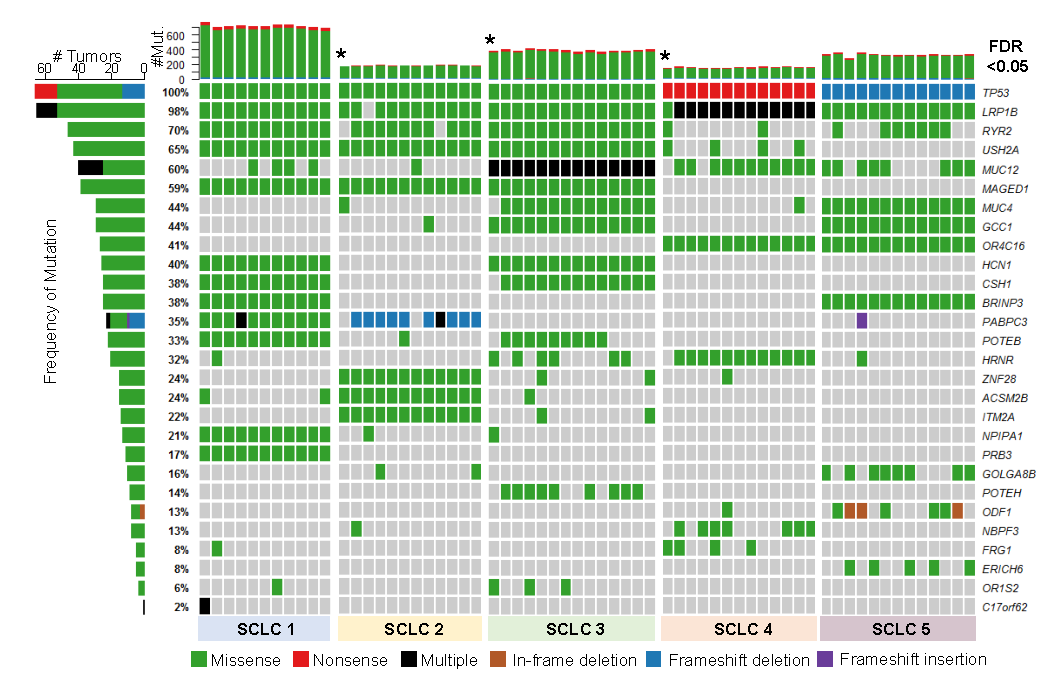
\includegraphics[width=0.9\textwidth,keepaspectratio]{images/sclc/oncoplot}
        \caption[Oncoplot of SMGs.]{Oncoplot of significantly mutated genes (SMGs) identified in our SCLC cohort using MuSiC (FDR $< 0.05$). Multiple tumor samples per SCLC patient were sequenced, resulting in exome data from 63 samples including 3 pre-treatment biopsy samples (marked by *). Vertical bar graphs (top) show total number of mutations per corresponding tumor sample below. Horizontal bar graphs and percentages (left) show mutational frequency of the corresponding gene (right). Type of somatic variant is defined by colored box key at the bottom, with black boxes indicating multiple variants detected in a specific gene in a given tumor sample.}
        \label{fig:sclc:oncoplot}
\end{figure}
WES revealed high tumor mutational burden (TMB) in our SCLC tumor samples, ranging from 5.7--29.8 mutations per megabase of genome (Supplemental Files~S\thechapter{}.2--6). The percentage of private somatic variants, or those present in only one tumor sample, in patients 1--5 ranged from 32--56\%, suggesting high intertumoral heterogeneity (Figure~\ref{fig:sclc:mutation_overview}). We assessed the identities of significantly mutated genes (SMGs) using MuSiC \cite{dees2012}, finding \textit{TP53} as the top SMG mutated in 100\% of tumor samples (Figure~\ref{fig:sclc:oncoplot}). Additional SMGs included \textit{LRP1B}, \textit{RYR2} and \textit{USH2A} (Supplemental File~S\thechapter{}.7). We sought to determine whether these genes may be preferentially mutated in SCLC relative to other cancer types by assessing their alteration frequency in the TCGA PanCancer Atlas studies (\textgreater{}10,000 samples) and 210 predominantly primary SCLC samples \cite{george2015,rudin2012,peifer2012,gardner2017} through cBioPortal for Cancer Genomics \cite{cerami2012,gao2013}. This analysis showed a high alteration frequency of these genes in SCLC but also in other cancer types with high TMB (Figure~\ref{fig:sclc:driver_bar_graphs}).

We detected an \textit{RB1} E204X nonsense mutation in a subset of tumor samples in patient 5 (Supplemental File~S\thechapter{}.6), and \textit{PTEN} mutations in patients 1 and 3. In patient 1, \textit{PTEN} C105F (a validated driver variant) was present in all metastatic tumor samples except for a residual primary right lung tumor and three brain metastases (Supplemental File~S\thechapter{}.2). In patient 3, \textit{PTEN} Y46N was present in a single metastatic tumor sample (Supplemental File~S\thechapter{}.4).

\begin{figure}[htb]
    \centering
    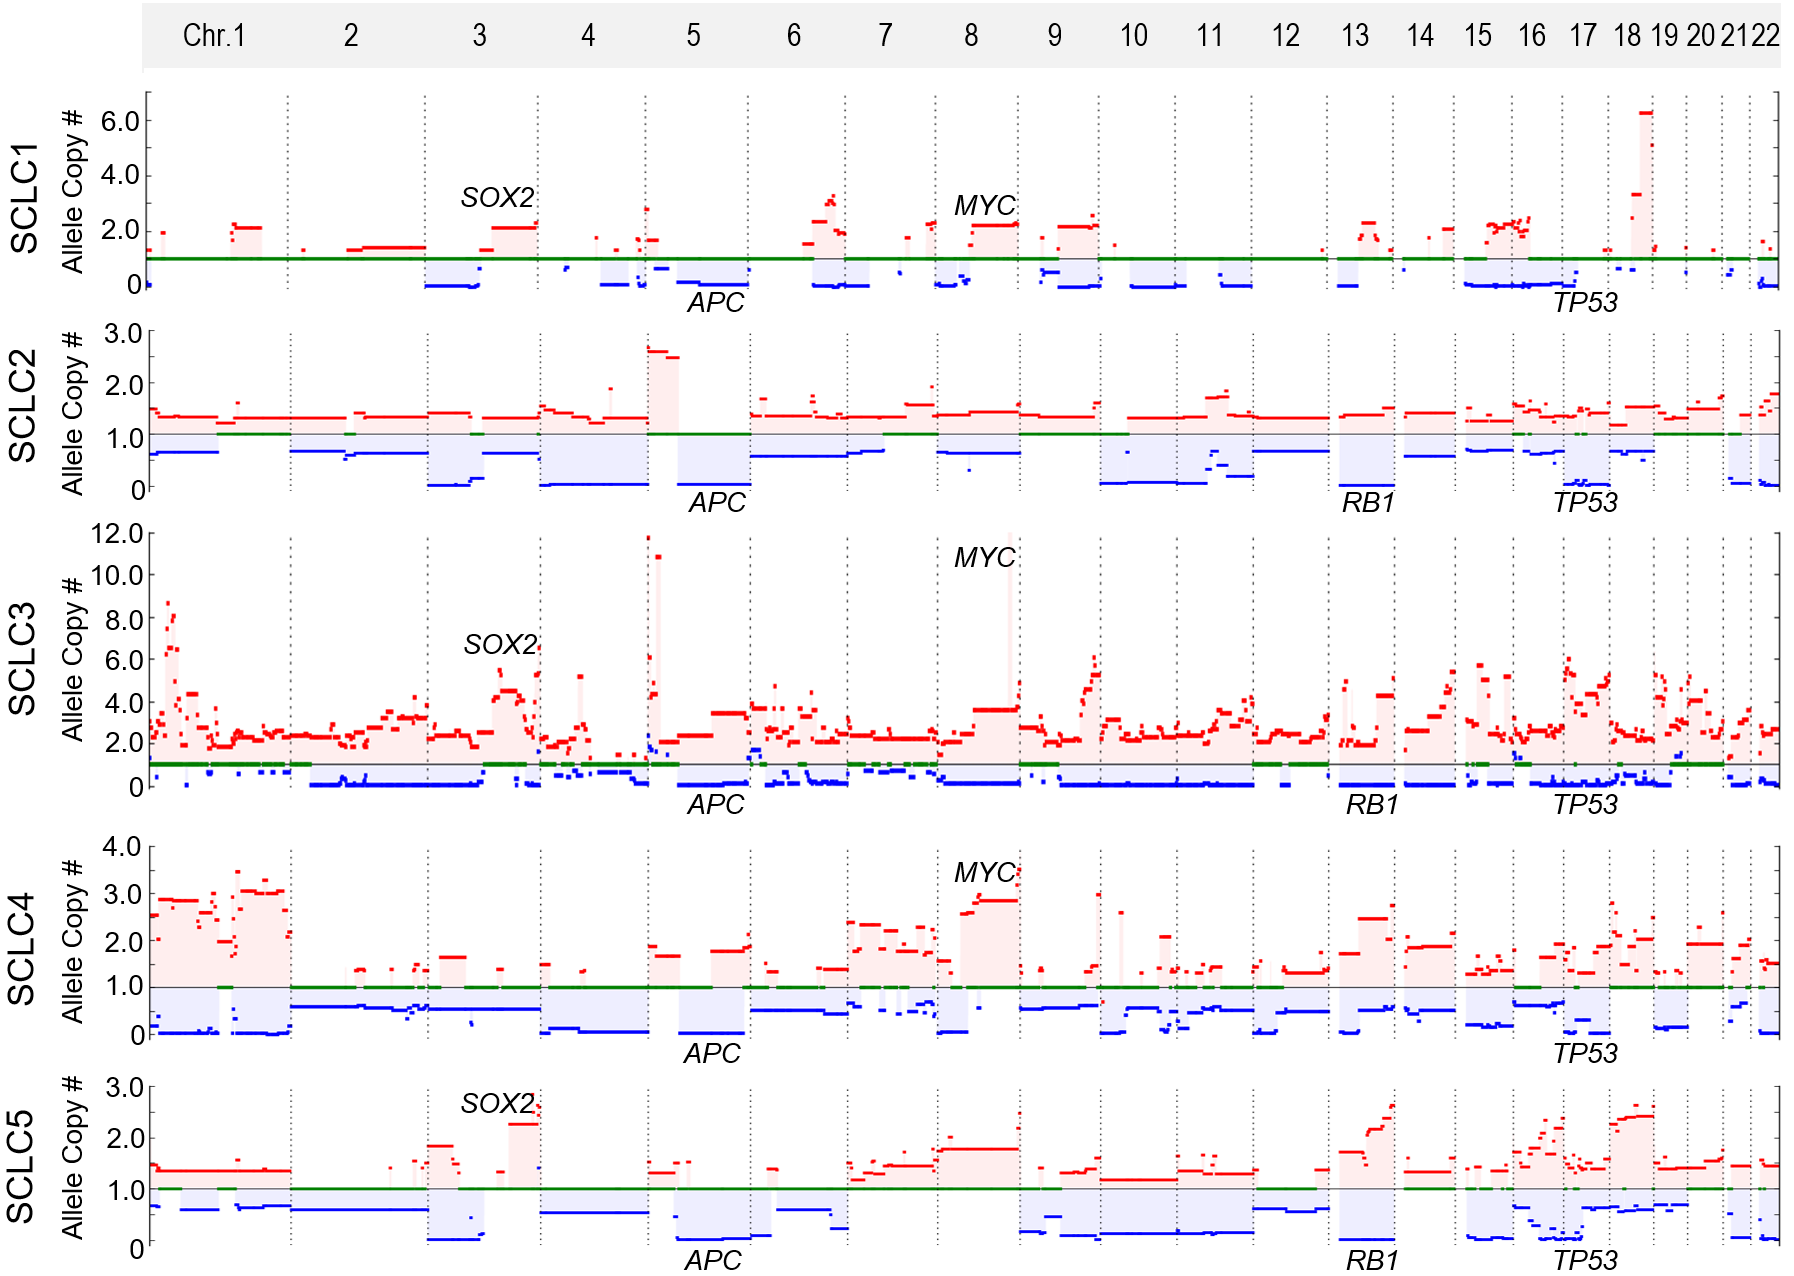
\includegraphics[width=0.9\textwidth,keepaspectratio]{images/sclc/cnv_plots}
    \caption[CNVs in SCLC autopsy patients.]{Uncurated CNVs in SCLC autopsy patients detected by FALCON\@. Data from all tumor samples per patient were pooled into a composite CNV profile as shown for each patient. Gains were defined as allele number $> 2.0$ (e.g.\ \textit{SOX2}) and loss $< 0.5$ (e.g.\ \textit{APC}). Red line, major allele. Blue line, minor allele. Green line, no change in one or both alleles.}
    \label{fig:sclc:cnv_plots}
\end{figure}
We identified a high frequency of CNVs using FALCON \cite{falcon} in all SCLC tumor samples from the five autopsy patients (Figure~\ref{fig:sclc:cnv_plots}, Supplemental File~S\thechapter{}.8). All patients demonstrated mono-allelic loss, defined as allele copy \textless{}0.5, of chromosome 17p regions containing \textit{TP53}. We also detected mono-allelic loss of chromosome 13q regions containing \textit{RB1} in patients 2, 3 and 5. Notably, tumor samples from all five patients had mono-allelic deletions of a region on chromosome 5q containing \textit{APC}. Consistent with previous studies \cite{rudin2012}, we detected allele-specific gains, defined as allele copy \textgreater{}2, of chromosome 3q regions containing \textit{SOX2} in patients 1, 3, and 5; and 8q regions containing \textit{MYC} in patients 1, 3, and 4. 

\subsection{Clonal heterogeneity and evolution in relapsed SCLC}
\begin{figure}[htbp]
    \centering
    \begin{subfigure}{0.85\textwidth}
        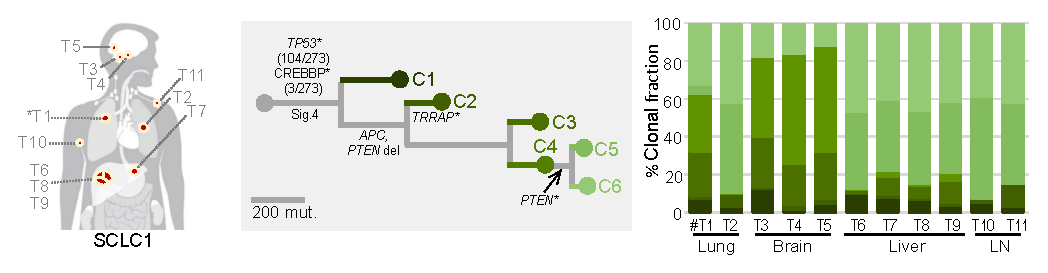
\includegraphics[width=\linewidth,keepaspectratio]{images/sclc/clones_sclc1}
        \vspace{-1cm}
        \caption{}\label{fig:sclc:clones_1}
    \end{subfigure}
    
    \vspace{0.5cm}
    \begin{subfigure}{0.85\textwidth}
        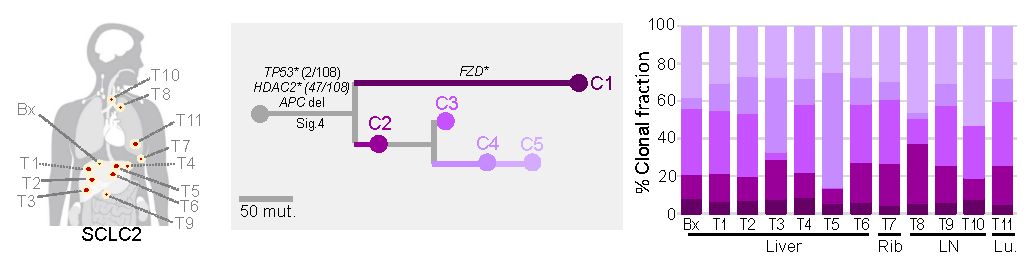
\includegraphics[width=\linewidth,keepaspectratio]{images/sclc/clones_sclc2}
        \vspace{-1cm}
        \caption{}\label{fig:sclc:clones_2}
    \end{subfigure}

    \vspace{0.5cm}
    \begin{subfigure}{0.85\textwidth}
        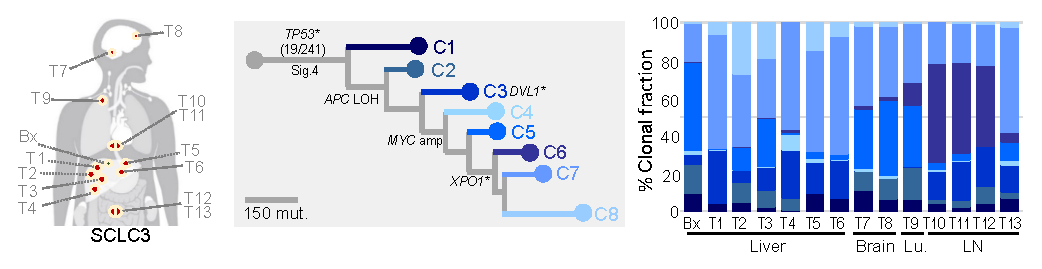
\includegraphics[width=\linewidth,keepaspectratio]{images/sclc/clones_sclc3}
        \vspace{-1cm}
        \caption{}\label{fig:sclc:clones_3}
    \end{subfigure}

    \vspace{0.5cm}
    \begin{subfigure}{0.85\textwidth}
        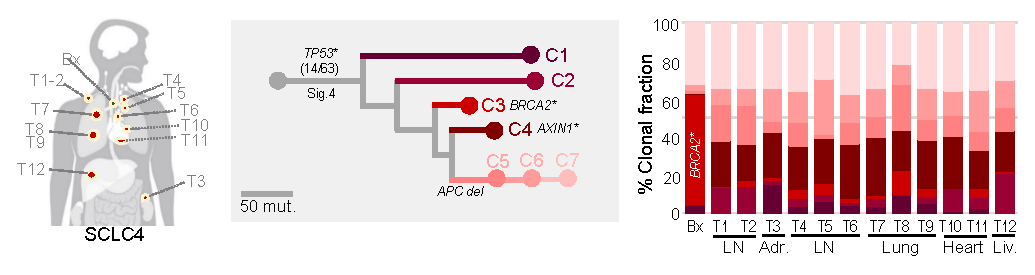
\includegraphics[width=\linewidth,keepaspectratio]{images/sclc/clones_sclc4}
        \vspace{-1cm}
        \caption{}\label{fig:sclc:clones_4}
    \end{subfigure}
    
    \vspace{-0.5cm}
    \caption[Clonal phylogeny and heterogeneity in four SCLC autopsy patients.]{Inferred clonal phylogeny and heterogeneity in four SCLC autopsy patients. Tumor samples procured from research autopsy as labeled on the human figure. Three large tumors from SCLC1 and SCLC3 were divided into multiple regions for sequencing. Phylogenetic trees depicting clonal evolution from a normal cell (gray solid circle) are shown, with branch length corresponding to mutational burden. Numbers in parentheses after genes show predicted order of occurrence in a truncal branch (e.g.\ (\subref{fig:sclc:clones_1}), \textit{CREBBP}, 3\textsuperscript{rd} mutation to occur out of 273 truncal alterations). The COSMIC tobacco mutation signature (Sig.\ 4) was detected in the trunk of all five phylogenetic trees. Clonal and subclonal predicted driver mutations, indicated by *, in Wnt signaling genes include \textit{CREBBP} and \textit{TRRAP} in SCLC1 (\subref{fig:sclc:clones_1}), \textit{FZD} in SCLC2 (\subref{fig:sclc:clones_2}), \textit{DVL1} and \textit{XPO1} in SCLC3 (\subref{fig:sclc:clones_3}), and \textit{AXIN1} in SCLC4 (\subref{fig:sclc:clones_4}). Percentages of different clones that compose each tumor sample are shown at right of each panel, demonstrating increased clonal heterogeneity. Bx, pre-treatment biopsy. LOH, loss of heterozygosity. \#T1, residual primary tumor in SCLC1.}
    \label{fig:sclc:clones_1234}
\end{figure}
We utilized the tool Canopy \cite{canopy} to integrate SNVs, indels and curated CNVs (Figure~\ref{fig:sclc:curated_cnv_plots}) to infer clonal diversity and architecture in advanced SCLC \cite{krook2019_mcs}. Between 5--8 genetically distinct tumor cell clones were inferred to exist in each patient (Figures~\ref{fig:sclc:clones_1234}, ~\ref{fig:sclc:clones_5}, Supplemental File~S\thechapter{}.9). \textit{TP53} and \textit{RB1} mutations were classified as truncal in all patients. Mutations in epigenetic modifiers such as \textit{CREBBP} and \textit{HDAC2} were also truncal, along with \textit{APC} (5q) deletion in a subset of patients. Subclonal alterations included \textit{PTEN} deletion and mutations as well as MYC amplification. We utilized CHASM \cite{carter2009} to identify predicted driver mutations in Wnt pathway genes such as \textit{XPO1} and \textit{AXIN1} (Supplemental File~S\thechapter{}.10). We utilized Bradley-Terry models to approximate the temporal occurrence of clonal and subclonal alterations and found that truncal alterations in \textit{TP53}, \textit{RB1}, \textit{CREBBP}, and \textit{HDAC2} occurred early, consistent with the critical role of these tumor suppressors in SCLC biology (Supplemental File~S\thechapter{}.11). Finally, we utilized deconstructSigs \cite{rosenthal16} to analyze mutational signatures and found truncal signature 4, which is known to be associated with tobacco smoking \cite{cosmic_ms}.

We next evaluated spatiotemporal clonal heterogeneity in advanced SCLC\@. In patient 1, we identified a tumor cell clone (Clone 4) unique to the brain metastases (T3--5) and the remnant primary tumor (*T1) (Figure~\ref{fig:sclc:clones_1}). In patient 2, the biopsy and post-treatment samples had similar clonal compositions (Figure~\ref{fig:sclc:clones_2}). In patient 3, clone 5 in the biopsy sample decreased significantly in all but three (T7--9) post-treatment tumors corresponding to brain and upper lung (Figure~\ref{fig:sclc:clones_3}). Conversely, clone 6 in the biopsy sample increased significantly in a subset of post-treatment tumors, particularly in the lymph node samples T10--12. In patient 4, clone 3 harboring a \textit{BRCA2} G620E mutation decreased significantly in all post-treatment tumor samples (T1--12) (Figure~\ref{fig:sclc:clones_4}), consistent with the well-characterized platinum-sensitizing effects of \textit{BRCA} mutations. Furthermore, post-treatment tumors had increased proportions of clones 4--6 that contained predicted driver alterations by CHASM in the Wnt pathway (\textit{AXIN1} mutation, \textit{APC} deletion), which has been associated with chemoresistance \cite{wagner2018}.

\begin{figure}[htbp]
    \centering
    \begin{subfigure}{0.85\textwidth}
        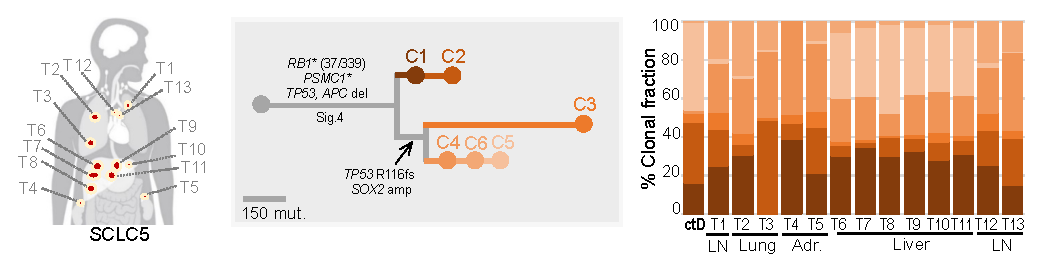
\includegraphics[width=\linewidth,keepaspectratio]{images/sclc/clones_sclc5}
        \vspace{-1cm}
        \caption{}\label{fig:sclc:clones_5}
    \end{subfigure}
    
    \hspace{0.1\textwidth}%
    \begin{subfigure}{0.35\textwidth}
        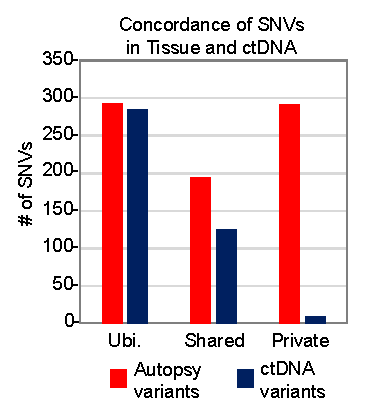
\includegraphics[width=\linewidth,keepaspectratio]{images/sclc/tissue_ctdna_concordance}
        \caption{}\label{fig:sclc:tissue_ctdna_concordance}
    \end{subfigure}%
    \hfill%
    \begin{subfigure}{0.35\textwidth}
        \vspace{0.08cm}
        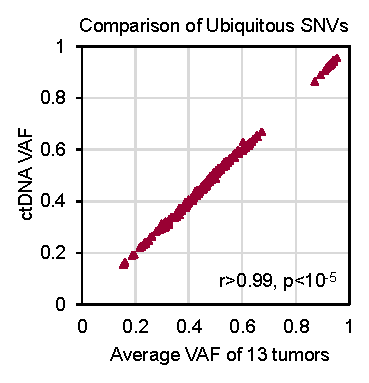
\includegraphics[width=\linewidth,keepaspectratio]{images/sclc/tissue_ctdna_ubiq}
        \vspace{0cm}
        \caption{}\label{fig:sclc:tissue_ctdna_ubiq}
    \end{subfigure}%
    \hspace{0.1\textwidth}
    
    \caption[Concordance between ctDNA and solid tumor in patient SCLC5.]{Concordance between circulating tumor DNA and tumor profiling in a fifth SCLC autopsy patient. (\subref{fig:sclc:clones_5}) Inferred clonal phylogeny and clonal composition of metastatic tumors from a fifth SCLC autopsy patient. Truncal predicted driver alterations include point mutations in \textit{RB1} and Wnt pathway gene \textit{PSMC1}, and copy number losses of \textit{TP53} and \textit{APC}. Tumor clonal heterogeneity was recapitulated in a circulating tumor DNA sample (ctD) collected shortly prior to death of this patient. The ctDNA sample showed a high proportion of Clone 5, which was detected in significant proportions only in the liver metastases T6-T11. (\subref{fig:sclc:tissue_ctdna_concordance}) Bar graph demonstrates concordant numbers of SNVs between tumor and ctDNA\@. (\subref{fig:sclc:tissue_ctdna_ubiq}) Average variant allele frequency (VAF) of ubiquitous SNVs compared with VAF of ctDNA variants.}
    \label{fig:sclc:patient_5}
\end{figure}
Finally, in patient 5, we identified a tumor cell clone (clone 5) present at increased proportions in all six liver metastases (T6--11; Figure~\ref{fig:sclc:clones_5}). Additionally, circulating tumor DNA (ctDNA) was isolated from the plasma of this patient shortly before death and subjected to WES (Supplemental File~S\thechapter{}.12). We determined high concordance ($p < 10^{-5}$) between ubiquitous tumor variants and ctDNA variants (Figure~\ref{fig:sclc:tissue_ctdna_concordance_detail}), including SNVs (Figures~\ref{fig:sclc:tissue_ctdna_concordance},~\ref{fig:sclc:tissue_ctdna_ubiq}) and indels. To infer the abundance of clones identified from autopsy in ctDNA, we utilized a maximum likelihood approach (Section~\ref{ssec:sclc:ctdna_clones}) that demonstrated similar clonal composition between ctDNA and the liver metastases (ctD,  Figure~\ref{fig:sclc:clones_5}), thus suggesting that this patient's hepatic tumor burden preferentially contributed to ctDNA\@.

\subsection[RNA sequencing reveals decreased anti-tumor immunity in SCLC]{RNA sequencing reveals decreased anti-tumor immunity in advanced SCLC}
To further characterize advanced SCLC, we performed transcriptome sequencing on a subset of tumor samples from each SCLC autopsy patient (Supplemental File~S\thechapter{}.1). Given the limited number of matched lung normal and pre-treatment\slash{}primary SCLC tumors in our data set, we incorporated additional publicly available SCLC RNA-seq data sets \cite{rudin2012,wagner2018,weiss2017,fagerberg2014} into all subsequent analyses. Two external SCLC data sets combined had 31 relapsed and 3 pre-treatment samples \cite{wagner2018,weiss2017}, one data set contained 30 primary SCLC and 25 matched normal samples \cite{rudin2012}, and one data set contained 8 normal lung samples \cite{fagerberg2014}. We first performed single sample GSEA (ssGSEA) \cite{barbie2009} using gene sets from the NanoString Tumor Signaling 360 panel (Supplemental File~S\thechapter{}.13). Intriguingly, most SCLC samples had decreased enrichment of pathways related to anti-tumor immune response: ``avoiding immune destruction'' and ``tumor-promoting inflammation'' compared to normal samples (Figure~\ref{fig:sclc:ssgsea_heatmap}).

\begin{figure}[htb]
    \centering
    \begin{subfigure}{0.84\textwidth}
        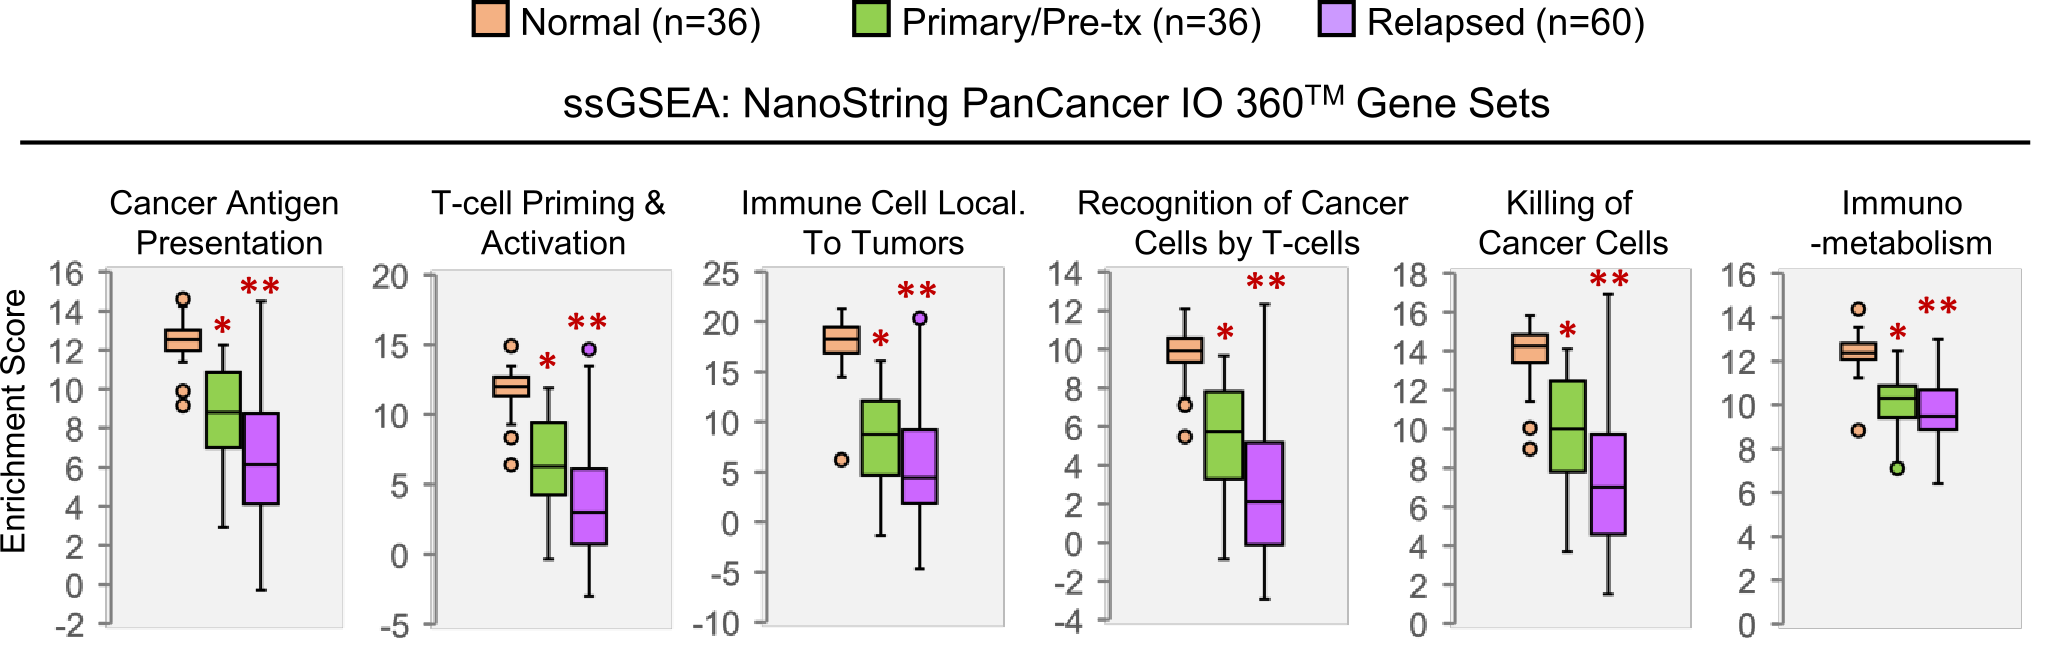
\includegraphics[width=\linewidth,keepaspectratio]{images/sclc/ssgsea_all_boxplot}
        \caption{}\label{fig:sclc:ssgsea_all_boxplot}
    \end{subfigure}
    
    \begin{subfigure}{0.84\textwidth}
        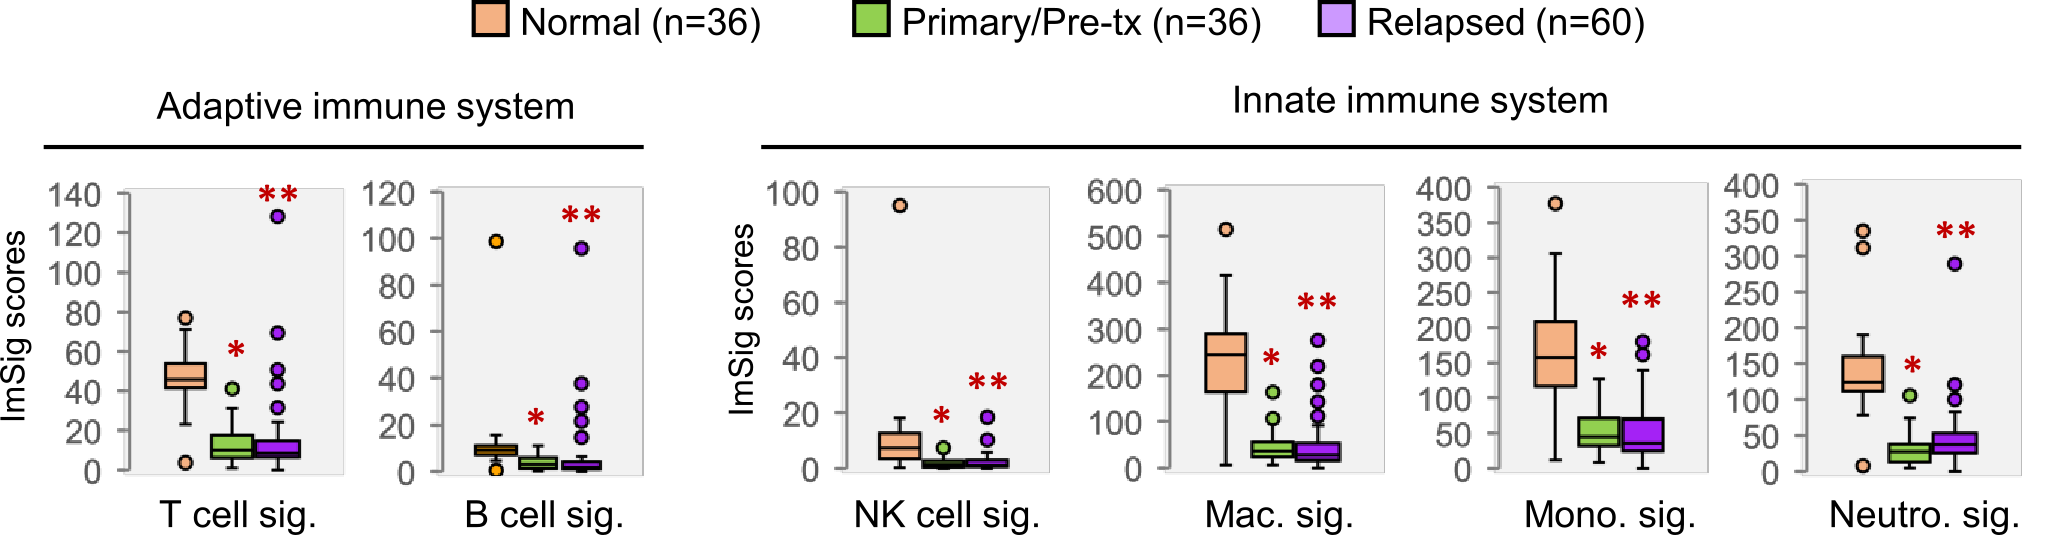
\includegraphics[width=\linewidth,keepaspectratio]{images/sclc/imsig_all_boxplot}
        \caption{}\label{fig:sclc:imsig_all_boxplot}
    \end{subfigure}
    \vspace{-0.5cm}
    \caption[Decreased expression of immune-associated genes in advanced SCLC.]{Transcriptome analyses reveal decreased expression of genes involved in anti-tumor immune responses in SCLC\@. (\subref{fig:sclc:ssgsea_all_boxplot}) Box plots of enrichment scores (ES) from ssGSEA analysis of gene sets derived from NanoString PanCancer IO 360 panel. Statistically significant differences in ES were detected in pairwise comparisons between normal-primary and normal-relapse. *: adjusted $p<0.0001$. (\subref{fig:sclc:imsig_all_boxplot}) Box plots of ImSig scores for different immune cell types in the adaptive and innate immune system. Statistically significant differences in ES were detected in pairwise comparisons between normal-primary and normal-relapse. *: adjusted $p<0.0001$.}
    \label{fig:sclc:immune_all_ssgsea_imsig}
\end{figure}
To delineate how the immune tumor microenvironment (TME) may be altered in SCLC, we next performed ssGSEA using the NanoString PanCancer Immuno-Oncology (IO) 360M panel. This showed decreased enrichment ($p < 0.001$) of processes annotated with adaptive anti-tumor immune function and immuno-metabolism in SCLC tumors relative to normal tissue (Figure~\ref{fig:sclc:ssgsea_all_boxplot}; Supplemental File~S\thechapter{}.13). We also utilized ImSig \cite{nirmal2018} to interrogate immune cell subsets in the SCLC TME, which showed low gene expression signatures of T cells and innate immune cells in primary and relapsed SCLC tumors (Figure~\ref{fig:sclc:imsig_all_boxplot}; Supplemental File~S\thechapter{}.13). Finally, we repeated ssGSEA and ImSig on our own research autopsy data set, in addition to above analyses of pooled data sets, and confirmed these results (Figure~\ref{fig:sclc:immune_rna_imsig})

\begin{figure}[htb]
    \centering
    \begin{subfigure}{0.84\textwidth}
        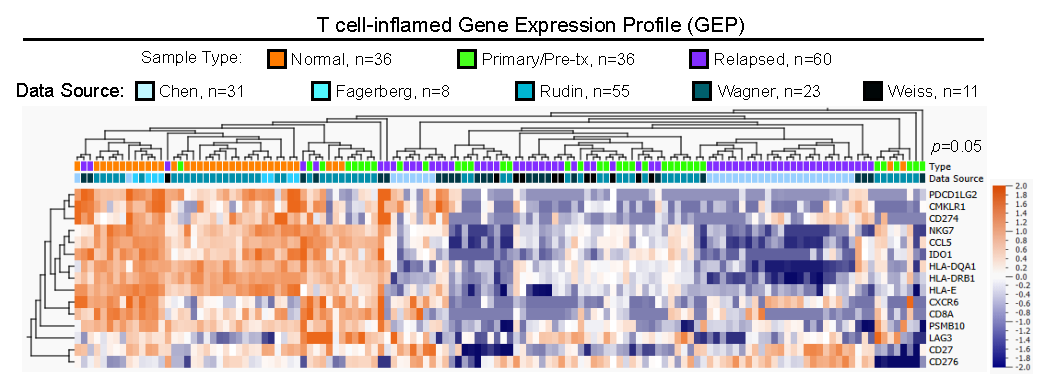
\includegraphics[width=\linewidth,keepaspectratio]{images/sclc/tis_genes_heatmap_sclc}
        \caption{}\label{fig:sclc:tis_genes_heatmap_sclc}
    \end{subfigure}
    
    \hspace{0.08\textwidth}%
    \begin{subfigure}{0.206\textwidth}
        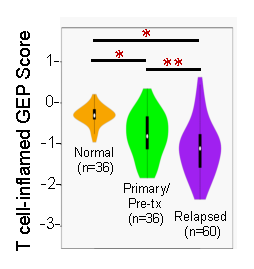
\includegraphics[width=\linewidth,keepaspectratio]{images/sclc/gep_violin_sclc}
        \caption{}\label{fig:sclc:gep_violin_sclc}
    \end{subfigure}%
    \hfill%
    \begin{subfigure}{0.584\textwidth}
        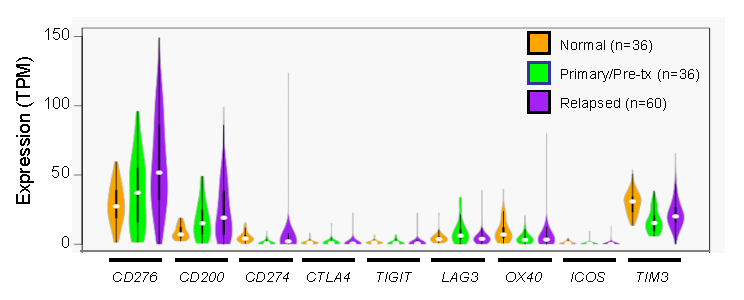
\includegraphics[width=\linewidth,keepaspectratio]{images/sclc/checkpoint_violin_sclc}
        \caption{}\label{fig:sclc:checkpoint_violin_sclc}
    \end{subfigure}%
    \hspace{0.08\textwidth}
    
    \vspace{-0.5cm}
    \caption[GEP evaluation reveals different immune phenotypes in neuroendocrine vs.\ non-neuroendocrine SCLC.]{T cell-inflamed gene expression profile (GEP) evaluation reveals different immune phenotypes in neuroendocrine versus non-neuroendocrine SCLC\@. (\subref{fig:sclc:tis_genes_heatmap_sclc}) Heat map of log transformed expression values (TPM) of genes representing the analytically validated T cell-inflamed GEP\@. Hierarchical clustering was performed using Qlucore Omics Explorer v3.6. Most primary and relapsed SCLC tumor samples demonstrated low GEP expression relative to normal lung tissue. Sample type and data source indicated as labeled. (\subref{fig:sclc:gep_violin_sclc}) Violin plot of GEP scores for normal, primary and relapsed SCLC samples. Higher scores indicate `hot' tumors, while lower scores indicate `cold' tumors. Two-tailed unpaired t-test. (\subref{fig:sclc:checkpoint_violin_sclc}) Violin plot of TPM values of selected T cell-inflamed GEP and checkpoint genes in normal and SCLC tumor samples. *, $p<0.001$. **, $p<0.005$.}
    \label{fig:sclc:immune_profiles}
\end{figure}
T cells are key mediators of the adaptive anti-tumor immune response and targets of immune checkpoint inhibitors (ICIs). Given that ssGSEA and ImSig results indicated decreased T cell presence in the SCLC TME, we further interrogated expression of eighteen genes in the analytically validated T cell-inflamed Gene Expression Profile (GEP), which was developed as a predictor of clinical benefit to ICI in multiple cancer types \cite{ayers2017}. Responders to ICI were shown to have pre-treatment baseline tumors with higher GEP scores (hot), whereas non-responders had tumors with lower baseline GEP scores (cold) \cite{cristescu2018,ayers2017}. Hierarchical clustering (Figure~\ref{fig:sclc:tis_genes_heatmap_sclc}) and calculation of GEP scores in the pooled (Figure~\ref{fig:sclc:gep_violin_sclc}) and autopsy only (Figure~\ref{fig:sclc:gep_violin_autopsy}) data sets demonstrated that most primary and relapsed SCLC are cold relative to either matched tissue normal or non-SCLC subtypes of adenocarcinoma and squamous cell carcinoma (Figure~\ref{fig:sclc:tis_genes_heatmap}, Supplemental File~S\thechapter{}.14). Only five SCLC tumors were inflamed and had GEP scores higher than the median score of \textapprox{}0.09 in normal samples (Supplemental File~S\thechapter{}.15).

As atezolizumab and durvalumab are both PD-L1 monoclonal antibodies approved in combination with chemotherapy in advanced SCLC, we examined the expression of PD-L1 (\textit{CD274}). \textit{CD274} expression was low in most primary and relapsed SCLC samples (Figures~\ref{fig:sclc:checkpoint_violin_sclc},~\ref{fig:sclc:checkpoint_violin_autopsy}), consistent with prior analyses showing that only a minority (\textapprox{}20\%) of SCLC patients had tumors with PD-L1 protein expression \textgreater{}1\% \cite{iams2020}. In contrast to \textit{CD274}, the expression of immune checkpoint inhibitory ligands \textit{CD276} (\textit{B7-H3}) and \textit{CD200} were increased in most SCLC tumor samples. Consistent with ImSig showing a lack of T cell signature in their TME, SCLC tumor samples had low expression levels of \textit{CTLA4}, \textit{TIGIT} and other immune checkpoint molecules found on T cells. Finally, interrogation of fifty SCLC cell lines from the Cancer Cell Line Encyclopedia (CCLE) recapitulated these gene expression patterns of \textit{CD276}, \textit{CD200} and \textit{CD274} (Figure~\ref{fig:sclc:checkpoint_violin_ccle}, Supplemental File~S\thechapter{}.14).

\begin{figure}[htb]
    \centering
    \begin{subfigure}{0.84\textwidth}
        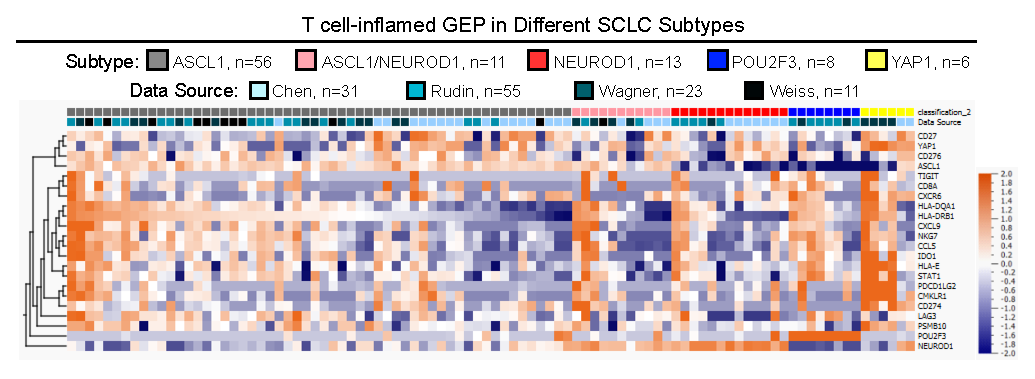
\includegraphics[width=\linewidth,keepaspectratio]{images/sclc/tis_genes_heatmap_sclc_subtype}
        \caption{}\label{fig:sclc:tis_genes_heatmap_sclc_subtype}
    \end{subfigure}
    
    \hspace{0.08\textwidth}%
    \begin{subfigure}{0.236\textwidth}
        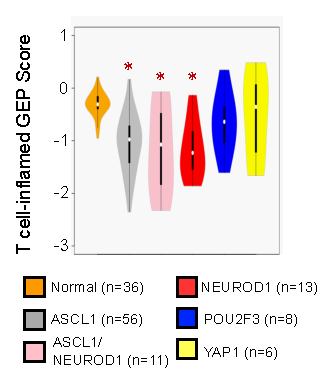
\includegraphics[width=\linewidth,keepaspectratio]{images/sclc/gep_violin_sclc_subtype}
        \caption{}\label{fig:sclc:gep_violin_sclc_subtype}
    \end{subfigure}%
    \hfill%
    \begin{subfigure}{0.304\textwidth}
        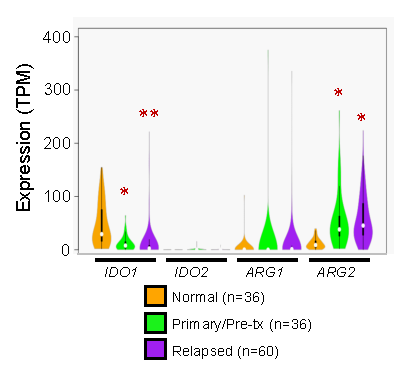
\includegraphics[width=\linewidth,keepaspectratio]{images/sclc/ido_arg_violin}
        \caption{}\label{fig:sclc:ido_arg_violin}
    \end{subfigure}%
    \hfill%
    \begin{subfigure}{0.250\textwidth}
        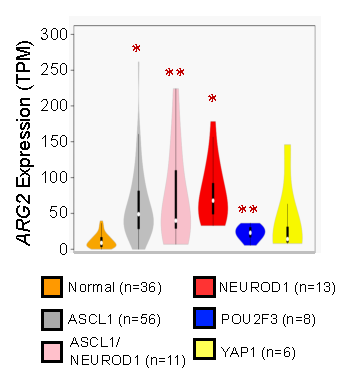
\includegraphics[width=\linewidth,keepaspectratio]{images/sclc/arg2_violin_subtype}
        \caption{}\label{fig:sclc:arg2_violin_subtype}
    \end{subfigure}%
    \hspace{0.08\textwidth}
    
    \vspace{-0.5cm}
    \caption[GEP evaluation by SCLC subtype.]{GEP evaluation by SCLC subtype. (\subref{fig:sclc:tis_genes_heatmap_sclc_subtype}) Heat map of log transformed expression values (TPM) of T cell-inflamed GEP genes in SCLC tumor samples annotated by subtype and data source as indicated. (\subref{fig:sclc:gep_violin_sclc_subtype}) Violin plot of GEP scores in different subtypes of SCLC and normal lung. Each subtype was compared against normal using two-tailed unpaired t-test. (\subref{fig:sclc:ido_arg_violin}) Violin plot of IDO1/2 and ARG1/2 expression in normal, primary and relapsed SCLC\@. Primary/pre-tx or relapsed samples were compared against normal using two-tailed unpaired t-test. (\subref{fig:sclc:arg2_violin_subtype}) Violin plot of ARG2 expression in SCLC tumor samples annotated by subtype. Each subtype was compared against normal using two-tailed unpaired t test. *, $p<0.001$. **, $p<0.005$.}
    \label{fig:sclc:immune_profiles_subtype}
\end{figure}
We further evaluated whether the four SCLC subtypes, as defined by the expression of \textit{ASCL1}, \textit{NEUROD1}, \textit{YAP1} and \textit{POU2F3} using a previously described method \cite{rudin2019} (Figure~\ref{fig:sclc:classification_scatter}) as well as based on highest gene expression evaluation (Supplemental File~S\thechapter{}.16), may have different immune phenotypes. As expected, most (n=56 of 94) SCLC samples were ASCL1-high, whereas tumors with high expression of \textit{ASCL1}/\textit{NEUROD1} (n=11), \textit{NEUROD1} (n=13), \textit{YAP1} (n=6) and \textit{POU2F3} (n=8) were the minority. Hierarchical clustering demonstrated that the non-neuroendocrine SCLC subtypes, YAP1 and POU2F3, had more tumors with elevated T cell-inflamed GEP while the classic and variant neuroendocrine subtypes were associated with predominantly low GEP (Figure~\ref{fig:sclc:tis_genes_heatmap_sclc_subtype}). When GEP scores were calculated for each subtype \cite{cristescu2018}, YAP1 and POU2F3 tumors had GEP scores closer to that of normal lung tissue (Figure~\ref{fig:sclc:gep_violin_sclc_subtype}). ImSig analysis further showed that YAP1 tumors, although limited in sample size, are particularly associated with increased T cell and innate immune cell signatures (Figure~\ref{fig:sclc:imsig_subtype_boxplot}).


\begin{figure}[htb]
    \centering
    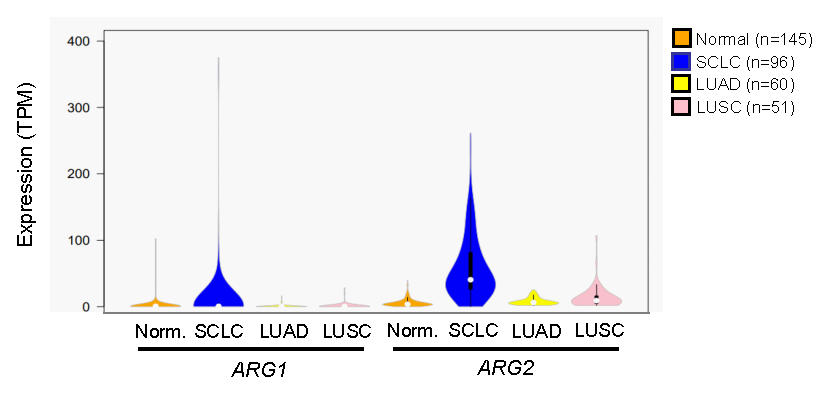
\includegraphics[width=0.9\textwidth,keepaspectratio]{images/sclc/arg_violin}
    \vspace{-0.5cm}
    \caption[Relative expression of \textit{ARG1} and \textit{ARG2}.]{Gene expression (TPM) of \textit{ARG1} and \textit{ARG2} in pooled normal lung, SCLC, lung adenocarcinoma (LUAD), and lung squamous cell carcinoma (LUSC)\@. Sample sizes are as indicated.}
    \label{fig:sclc:arg_violin}
\end{figure}
Finally, to extend our analysis of suppressed immune function in SCLC, we interrogated expression of immunometabolism genes (Figure~\ref{fig:sclc:ssgsea_all_boxplot}) encoding indoleamine 2,3-dioxygenase (IDO1/2) and arginase (ARG1/2) enzymes (Figure~\ref{fig:sclc:ido_arg_violin}), whose metabolic function have been shown to inhibit effector T cell and NK cell activity \cite{osullivan2019,wang2012,grzywa2020}. Out of the four genes, only \textit{ARG2} expression was significantly increased in primary and relapsed SCLC tumors and cell lines (Figure~\ref{fig:sclc:checkpoint_violin_ccle}). We then evaluated \textit{ARG2} expression based on SCLC subtypes (Figure~\ref{fig:sclc:arg2_violin_subtype}) and in NSCLC (Figures~\ref{fig:sclc:tis_genes_heatmap}). This analysis showed high \textit{ARG2} expression in the neuroendocrine SCLC subtypes (ASCL1, ASCL1/NEUROD1, and NEUROD1) and low \textit{ARG2} expression in the non-neuroendocrine subtypes (YAP1 and POU2F3), as well as low \textit{ARG2} expression in NSCLC (Figure~\ref{fig:sclc:arg_violin}). Taken together, these results support the need to further investigate \textit{ARG2} as a potential negative regulator of immune TME in the most common neuroendocrine SCLC subtypes.

\section{Discussion}
In this study, we leveraged rapid research autopsy to perform genomic and transcriptomic characterization of advanced SCLC\@. Our results demonstrated substantial clonal heterogeneity in relapsed SCLC, arising through branching and linear evolution. We identified numerous subclonal alterations likely underlying treatment-sensitivity, thus explaining the expansion or reduction of specific clones in tumors at different metastatic sites in each patient. Although limited in sample size, our results showed that certain clones are enriched in metastatic sites such as brain and liver, with liver as the main ctDNA contributor in one patient. The ability to detect tissue-specific clones may have certain clinical utility. For example, the central nervous system (CNS) is a frequent site of metastasis in SCLC patients. The presence of brain-specific subclonal alterations in the ctDNA may help predict which patients are at highest risk for CNS disease and therefore be considered for prophylactic cranial irradiation or novel therapies to prevent CNS disease. Our study demonstrates the utility of autopsy in studying subclone preference for specific metastatic niches, which will require additional autopsies of patients with SCLC and other solid tumors.

In addition to identifying \textit{TP53} as the top SMG and inferring \textit{TP53} mutations as truncal drivers in all autopsy patients, we also identified multiple mutations in \textit{LRP1B}, which has putative tumor suppressor functions \cite{beer2016,prazeres2011,wang2017}. These truncal alterations raise the possibility that \textit{LRPB1}-mutant tumor cells may acquire an early fitness advantage over wild-type cells, which is further supported by an increased frequency of \textit{LRP1B} mutations in primary SCLC tumor samples (Figure~\ref{fig:sclc:mutation_heatmaps}). Thus, we propose that functional validation of variants in this gene and others (e.g. \textit{RYR2}, \textit{USH2A}) in appropriate model systems may begin to unravel their roles in the biology of SCLC and potentially other cancers.

Alterations in the Wnt signaling pathway have been linked to acquired chemoresistance in relapsed SCLC \cite{wagner2018}. In a cohort of thirty relapsed SCLC samples, loss of heterozygosity of either \textit{APC} or \textit{CDH8} was detected in 23/30 samples, while mutations in either gene were detected in 10/30 samples. In our autopsy cohort, we identified copy number loss of APC as truncal or very early subclonal events in patients 1--3. We found truncal (\textit{PSMC1}) and multiple subclonal (\textit{TRRAP}, \textit{FZD2}, and \textit{XPO1}) predicted driver mutations in other Wnt signaling pathway genes. For instance, in patient 3, the autopsy tumor samples were enriched for clones C6--C8 containing an \textit{XPO1} mutation. In patient 4, mutation of another Wnt signaling gene, \textit{AXIN1}, was assigned to a clone of tumor cells (C4) exclusively detected in post-treatment autopsy tumor samples. Therefore, our results are consistent with and support the established association between Wnt pathway and early chemoresistance in advanced SCLC\@.

Analysis of ctDNA in advanced SCLC patients represents a valuable approach to tracking tissue-specific clones or emergence of resistant clones \cite{nong2018}. While most studies have compared ctDNA to either a single primary or metastatic tumor biopsy, rapid autopsy enables the comparison of variants detected in ctDNA against variants in multiple metastatic tumors. In our study, we performed WES of ctDNA from patient 5 and detected nearly all ubiquitous tumor variants from autopsy that likely represented the majority of this patient's truncal variants (concordance 97--100\% for SNVs and indels). Not surprisingly, for variants that were classified as shared or private at autopsy (\textit{e.g.}\ subclonal variants), the metastatic tumor-ctDNA concordance rates were significantly lower. Therefore, our results show effective detection of truncal variants in ctDNA, but considerable limitations for detecting subclonal variants. These data and future autopsy studies will provide significant contributions towards refining the limits of ctDNA detection for clinical applications, including the evaluation of minimal residual disease and cancer recurrence.

Within our autopsy SCLC cohort, we performed transcriptome sequencing to evaluate whether mutations in SMGs may correlate with altered expression, thereby representing potential driver genes. However, this initial analysis did not reveal a significant correlation. Additionally, consistent with prior studies showing a paucity of gene fusions as drivers in SCLC \cite{iwakawa2013}, we did not detect any putative fusions that were recurrent in more than one tumor sample within our cohort. Recognizing that these results may be attributed to our limited cohort size, we incorporated external primary and relapsed SCLC RNA-seq data sets in subsequent analyses, which ultimately revealed suppressed immune TME in the neuroendocrine SCLC subtypes (ASCL1, NEUROD1, and ASCL1/NEUROD1).

Given that only \textapprox{}20\% of SCLC patients have tumors expressing PD-L1 (\textgreater{}1\% by immunohistochemistry) \cite{iams2020}, improved characterization of the SCLC immune TME remains an unmet need, particularly given recent regulatory approvals of front-line PD-L1 blockade therapy. Our results confirmed low \textit{CD274} (PD-L1) expression in most SCLC tumors and cell lines, supporting the above clinical observations. Additional ssGSEA and ImSig analyses corroborated decreased adaptive anti-tumor immune function in primary and relapsed SCLC\@. Although we lacked outcomes data to correlate with T cell-inflamed GEP scores, which predicts clinical benefit to PD-1/PD-L1 blockade \cite{gao2013}, hierarchical clustering revealed a non-inflamed phenotype in most primary and advanced SCLC\@. Interestingly, T cell-inflamed GEP expression was high, or close to that of normal lung samples, in non-neuroendocrine SCLC subtypes (YAP1 and POU2F3) (Figure~\ref{fig:sclc:tis_genes_heatmap_sclc_subtype}), which had low \textit{ARG2} expression (Figure~\ref{fig:sclc:gep_violin_sclc_subtype}). In contrast, GEP expression was low in the neuroendocrine SCLC subtypes (ASCL1, ASCL1/NEUROD1, and NEUROD1), which had high \textit{ARG2} expression. Given these observations, we hypothesize that increased arginase 2 expression and function may represent a cell-autonomous oncogenic metabolic adaptation enabling suppression of adaptive anti-tumor immunity in the SCLC TME independent of PD-L1 expression. These results will need to be validated in larger, independent data sets, but suggest that subtyping SCLC patients prior to systemic treatment should aid in the identification of patients most likely to benefit from chemo-ICI\@. Finally, it was recently reported that the non-neuroendocrine SCLC subtypes were more likely to be admixed SCLC and NSCLC \cite{baine2020}, which in addition to low \textit{ARG2} expression, may further explain the higher GEP scores and inflamed phenotype in these tumors given the responsiveness of NSCLC to ICI\@.

Continuing the analysis of immune TME, in addition to decreased \textit{CD274} expression, we showed decreased expression of \textit{CTLA4}, \textit{LAG3}, \textit{TIM3}, and other well-characterized immune checkpoint proteins in advanced SCLC\@. Conversely, we detected increased expression of alternate checkpoint molecules, \textit{CD276} (B7-H3) and \textit{CD200}. \textit{CD276} is a member of the B7 family, which also includes PD-L1 (B7-H1). Consistent with our finding of increased gene expression, \textit{CD276} protein expression was recently detected in 64.9\% of a SCLC cohort with ninety patients \cite{carvajalhausdorf2019}. The same study reported PD-L1 expression at a much lower rate of 7.3\%. \textit{CD276} is expressed at low levels in normal tissues but when aberrantly expressed on various tumor cell types contributes to T cell inhibition, tumor cell immune evasion, and is associated with poor prognosis \cite{dong2018}. Therefore, targeting CD276 is being explored as an immune-stimulatory strategy in cancer \cite{picarda2016}. CD200 is a checkpoint molecule that leads to suppression of secretion of pro-inflammatory cytokines, including IL-2 and IFN$\gamma$ \cite{xiong2020}. Consistent with increased CD200 expression in the SCLC samples we analyzed, CD200 protein was expressed in two other SCLC cohorts \cite{bohling2015,love2017}. Furthermore, inhibiting the CD200 signaling axis has been shown to significantly stimulate antigen-specific immune response against glioblastoma multiforme \cite{xiong2020}. Therefore, these results support further exploration of targeting CD276 or CD200 in pre-clinical SCLC models to determine whether inhibiting these checkpoint pathways may yield viable therapeutic strategies for advanced SCLC\@.

As drug development efforts focus on PD-1/PD-L1 and other immune regulatory checkpoints, characterization of both the immune microenvironment and tumor heterogeneity will be critical to differentiate responders from non-responders. It will also be important to define the relationship between tumor heterogeneity and neoantigen formation. For example, in NSCLC, cytotoxic tumor-infiltrating T cells preferentially develop against clonal neoantigens (derived from clonal or truncal mutations) in patients with durable clinical benefit to ICI \cite{mcgranahan2016}. The high smoking-associated TMB of SCLC suggests that there may a high number of clonal neoantigens serving as therapeutic targets. Therefore, a combination of autopsy and ctDNA samples will be critical resources to help characterize the prevalence of clonal neoantigens and optimize their detection from liquid biopsy. This will enable the development vaccine or T cell-based therapeutic strategies in SCLC and other solid cancers.

In summary, we have partnered with patients for rapid research autopsy to study relapsed SCLC and performed extensive analyses of clonal heterogeneity, subclonal architecture, and the immune microenvironment. Our results suggest a potential explanation for why SCLC, a cancer with high TMB and thus potential tumor neoantigens, exhibits lower than expected response rates to ICI compared to other solid tumors with similar median TMB\@. Future studies employing single-cell sequencing strategies will shed light on unanswered questions, including which cell types are the source of \textit{ARG2} expression and whether \textit{CD200}/\textit{CD276} are co-expressed. Metabolome profiling could identify additional metabolic vulnerabilities in SCLC that may be co-targeted to enhance ICI response. Innovative immunotherapeutic approaches targeting alternate checkpoints, potentially combined with isoform-specific arginase inhibition, may ultimately result in more robust clinical activity against advanced SCLC\@.

\section{List of Supplemental Files}
All supplemental files are available at \url{https://github.com/rbonneville/PhD-Dissertation/}.
\begin{enumerate}
    \renewcommand*{\labelenumi}{S\thechapter{}.\arabic{enumi}. }
    \item Next generation sequencing summary of 69 total WES samples and 32 RNA-seq samples from 5 SCLC autopsy patients. For each tumor or normal sample, the anatomical site, pathologist estimate of \% tumor cell content, median/average sequencing coverage, and \% of exonic bases covered at least 100\texttimes{} are reported. For WES, SNPs and indels were called using VarScan2, and Tumor Mutational Burden (TMB) reported as mutations/megabase of sequence.
    \item VAFs of all somatic mutations (SNPs and indels) within patient SCLC1\@. Listed coordinates are in hg19. Variants were annotated using ANNOVAR\@.
    \item VAFs of all somatic mutations (SNPs and indels) within patient SCLC2\@. Listed coordinates are in hg19. Variants were annotated using ANNOVAR\@.
    \item VAFs of all somatic mutations (SNPs and indels) within patient SCLC3\@. Listed coordinates are in hg19. Variants were annotated using ANNOVAR\@.
    \item VAFs of all somatic mutations (SNPs and indels) within patient SCLC4\@. Listed coordinates are in hg19. Variants were annotated using ANNOVAR\@.
    \item VAFs of all somatic mutations (SNPs and indels) within patient SCLC5\@. Listed coordinates are in hg19. Variants were annotated using ANNOVAR\@.
    \item Variants and VAFs in Significantly Mutated Genes from 5 SCLC patients detected using MuSiC v2.0.
    \item Raw and curated CNV calls for all tumor samples from 5 SCLC autopsy patients. Allele-specific CNVs were called using FALCON and manually curated. For sample key, please refer to Supplemental File~S\thechapter{}.1.
    \item Estimated fraction of each clone and normal cells within tumor samples as determined by Canopy. For patient 5, the estimated clonal and normal fractions as detected in ctDNA by our statistical optimization approach are also reported. For sample key, please refer to Supplemental File~S\thechapter{}.1.
    \item List of canonical Wnt signaling genes and Wnt signaling genes with mutations in 5 SCLC autopsy patients. Wnt gene mutations were further classified as non-driver or driver mutations using CHASM\@. For sample key, please refer to Supplemental File~S\thechapter{}.1.
    \item Ordered mutations (SNVs and indels), CNVs and mutational signatures within each branch of the phylogenetic trees from 5 SCLC autopsy patients. Clones and phylogenetic trees were inferred by Canopy, and remaining mutations were assigned to the tree via a maximal likelihood model. Signatures from mutational groups with fewer than 50 SNVs are italicized, as at least 50 mutations are recommended for input to deconstructSigs. For sample key, please refer to Supplemental File~S\thechapter{}.1.
    \item Variants (SNVs and indels), raw CNV output and curated CNV data from ctDNA sequencing in patient 5. Mutations labeled as ``Ubiquitous'' were detected in all 13 tissue samples from this patient, ``Shared'' from 2 to 12 samples, ``Private'' from 1 sample, and ``ctDNA only'' from 0 tumor samples. CNV curation was performed using the regions determined from tissue samples (see Supplemental File~S\thechapter{}.8).
    \item Single sample GSEA enrichment scores and ImSig scores in normal tissue, primary and relapsed SCLC\@. ssGSEA analysis was performed using NanoString Tumor Signaling 360 and PanCancer IO 360 gene sets; positive and negative scores correlate with direction of enrichment. ImSig scores were generated for adaptive and innate immune cell types.
    \item Gene expression TPM values for 18 genes in the T cell-inflamed GEP and ARG1/2 in SCLC and TCGA NSCLC samples. TCGA sample IDs are included. TPM values for all genes in NanoString PanCancer IO 360 panel are provided for the 50 SCLC cell lines from the Cancer Cell Line Encyclopedia. 
    \item Calculation of T cell-inflamed GEP scores in SCLC tumor samples.
    \item Molecular subtyping of primary and relapsed SCLC samples based on expression of \textit{ASCL1}, \textit{NEUROD1}, \textit{YAP1}, and \textit{POU2F3}.
\end{enumerate}

\section*{Acknowledgements}
We are grateful for technical advice and support for NextSeq sequencing from Dr.\ Dara Aisner in the Department of Pathology at the University of Colorado School of Medicine; Drs.\ Eric Haura and Theresa Boyle at Moffitt Cancer Center (Tampa, FL) for critical reading of the manuscript; excellent administrative support from Jenny Badillo, the Genomics Shared Resource at The Ohio State University Comprehensive Cancer Center, the Ohio Supercomputer Center, community support from Pelotonia, as well as patients and their families for their participation in cancer research. The results published here are in part based upon data generated by the TCGA Research Network: \url{https://www.cancer.gov/tcga}.